\documentclass[twocolumn,10pt]{asme2ej}

\usepackage{epsfig} 

\title{Objektvermessung mit OpenCV}

\author{Tobias Rohrer
    \affiliation{
	Hochschule Darmstadt\\
	Data Science (Master)\\
    Email: Tobias.Rohrer@outlook.com
    }	
}

\graphicspath{ {./images/} }
\usepackage[center]{caption}
\usepackage[locale=DE]{siunitx}

\usepackage{listings}
\usepackage{xcolor}

\definecolor{codegreen}{rgb}{0,0.6,0}
\definecolor{codegray}{rgb}{0.5,0.5,0.5}
\definecolor{codepurple}{rgb}{0.58,0,0.82}
\definecolor{backcolour}{rgb}{0.95,0.95,0.92}

\lstdefinestyle{mystyle}{
	backgroundcolor=\color{backcolour},   
	commentstyle=\color{codegreen},
	keywordstyle=\color{magenta},
	numberstyle=\tiny\color{codegray},
	stringstyle=\color{codepurple},
	basicstyle=\ttfamily\footnotesize,
	breakatwhitespace=false,         
	breaklines=true,                 
	captionpos=b,                    
	keepspaces=true,                 
	numbers=left,                    
	numbersep=5pt,                  
	showspaces=false,                
	showstringspaces=false,
	showtabs=false,                  
	tabsize=2
}
\lstset{style=mystyle}
\begin{document}

\maketitle    

%%%%%%%%%%%%%%%%%%%%%%%%%%%%%%%%%%%%%%%%%%%%%%%%%%%%%%%%%%%%%%%%%%%%%%
\begin{abstract}
{\it Die maschinelle Vermessung von metallischen Gegenständen ist durch spiegelnde Materialeigenschaften komplex. Es wurde eine Softwarelösung für die Vermessung in Python mit der \emph{OpenCV}-Bibliothek\cite{opencv_library} entworfen und implementiert. Die Umrechnung der Kantenlängen von Pixel in Millimeter wurde durch das Platzieren eines Referenzobjekt mit bekannten Maßen ermöglicht. Durch den Einsatz eines Hintergrundes mit hohem Kontrast, sowie der Wahl von günstigen Belichtungsverhältnissen konnte die Robustheit des Verfahrens verbessert werden. Der durchschnittliche Messfehler beträgt 1.1\%.
}
\end{abstract}

%%%%%%%%%%%%%%%%%%%%%%%%%%%%%%%%%%%%%%%%%%%%%%%%%%%%%%%%%%%%%%%%%%%%%%
\section{Einleitung}
Die genaue Vermessung von Werkstücken ist in der Qualitätssicherung von zentraler Rolle. Mit Hilfe von maschinellem Sehen kann dieser Schritt automatisiert werden. Doch die Vermessung von metallischen Objekten stellt sich auf Grund von spiegelnden optischen Eigenschaften fehleranfällig dar. In der vorliegenden Arbeit wird die Implementierung eines Vermessungssystems mit Hilfe der \emph{OpenCV}-Bilbliothek beschrieben. 

Das entworfene und implementierte Verfahren stützt sich auf den Grundideen aus \cite{PyImageSearch}. Hier wird ein Vorgehen zur Objektvermessung mit der  \emph{OpenCV}-Bilbliothek beschrieben. Abzugrenzen ist diese Arbeit von \cite{PyImageSearch} durch Änderungen in den Vorbereitungsschritten, wodurch das Verfahren auf metallische Objekte mit spiegelnden Eigenschaften ausgeweitet werden konnte. Des Weiteren konnte gezeigt werden, dass der Vorverarbeitungsschritt mit Hilfe des \emph{Canny Edge Detectors}\cite{Canny} für diesen Anwendungsfall nicht Notwendig ist.

\section{Konzeption}\label{sec:2}
Für eine genaue Vermessung sind die Aufnahmebedingungen beim Erstellen des Bildmaterials entscheidend. Es soll deshalb ein dunkler Hintergrund verwendet werden, um die Auswirkungen von Schatten möglichst gering zu halten. Außerdem entsteht dadurch ein guter Kontrast zwischen dem dunklen Bildhintergrund und den metallischen Objekten. Es muss des Weiteren darauf geachtet werden, dass alle Bilder mit einem \ang{90} Winkel aufgenommen werden, um Verzerrungen zu vermeiden.

\begin{figure}
	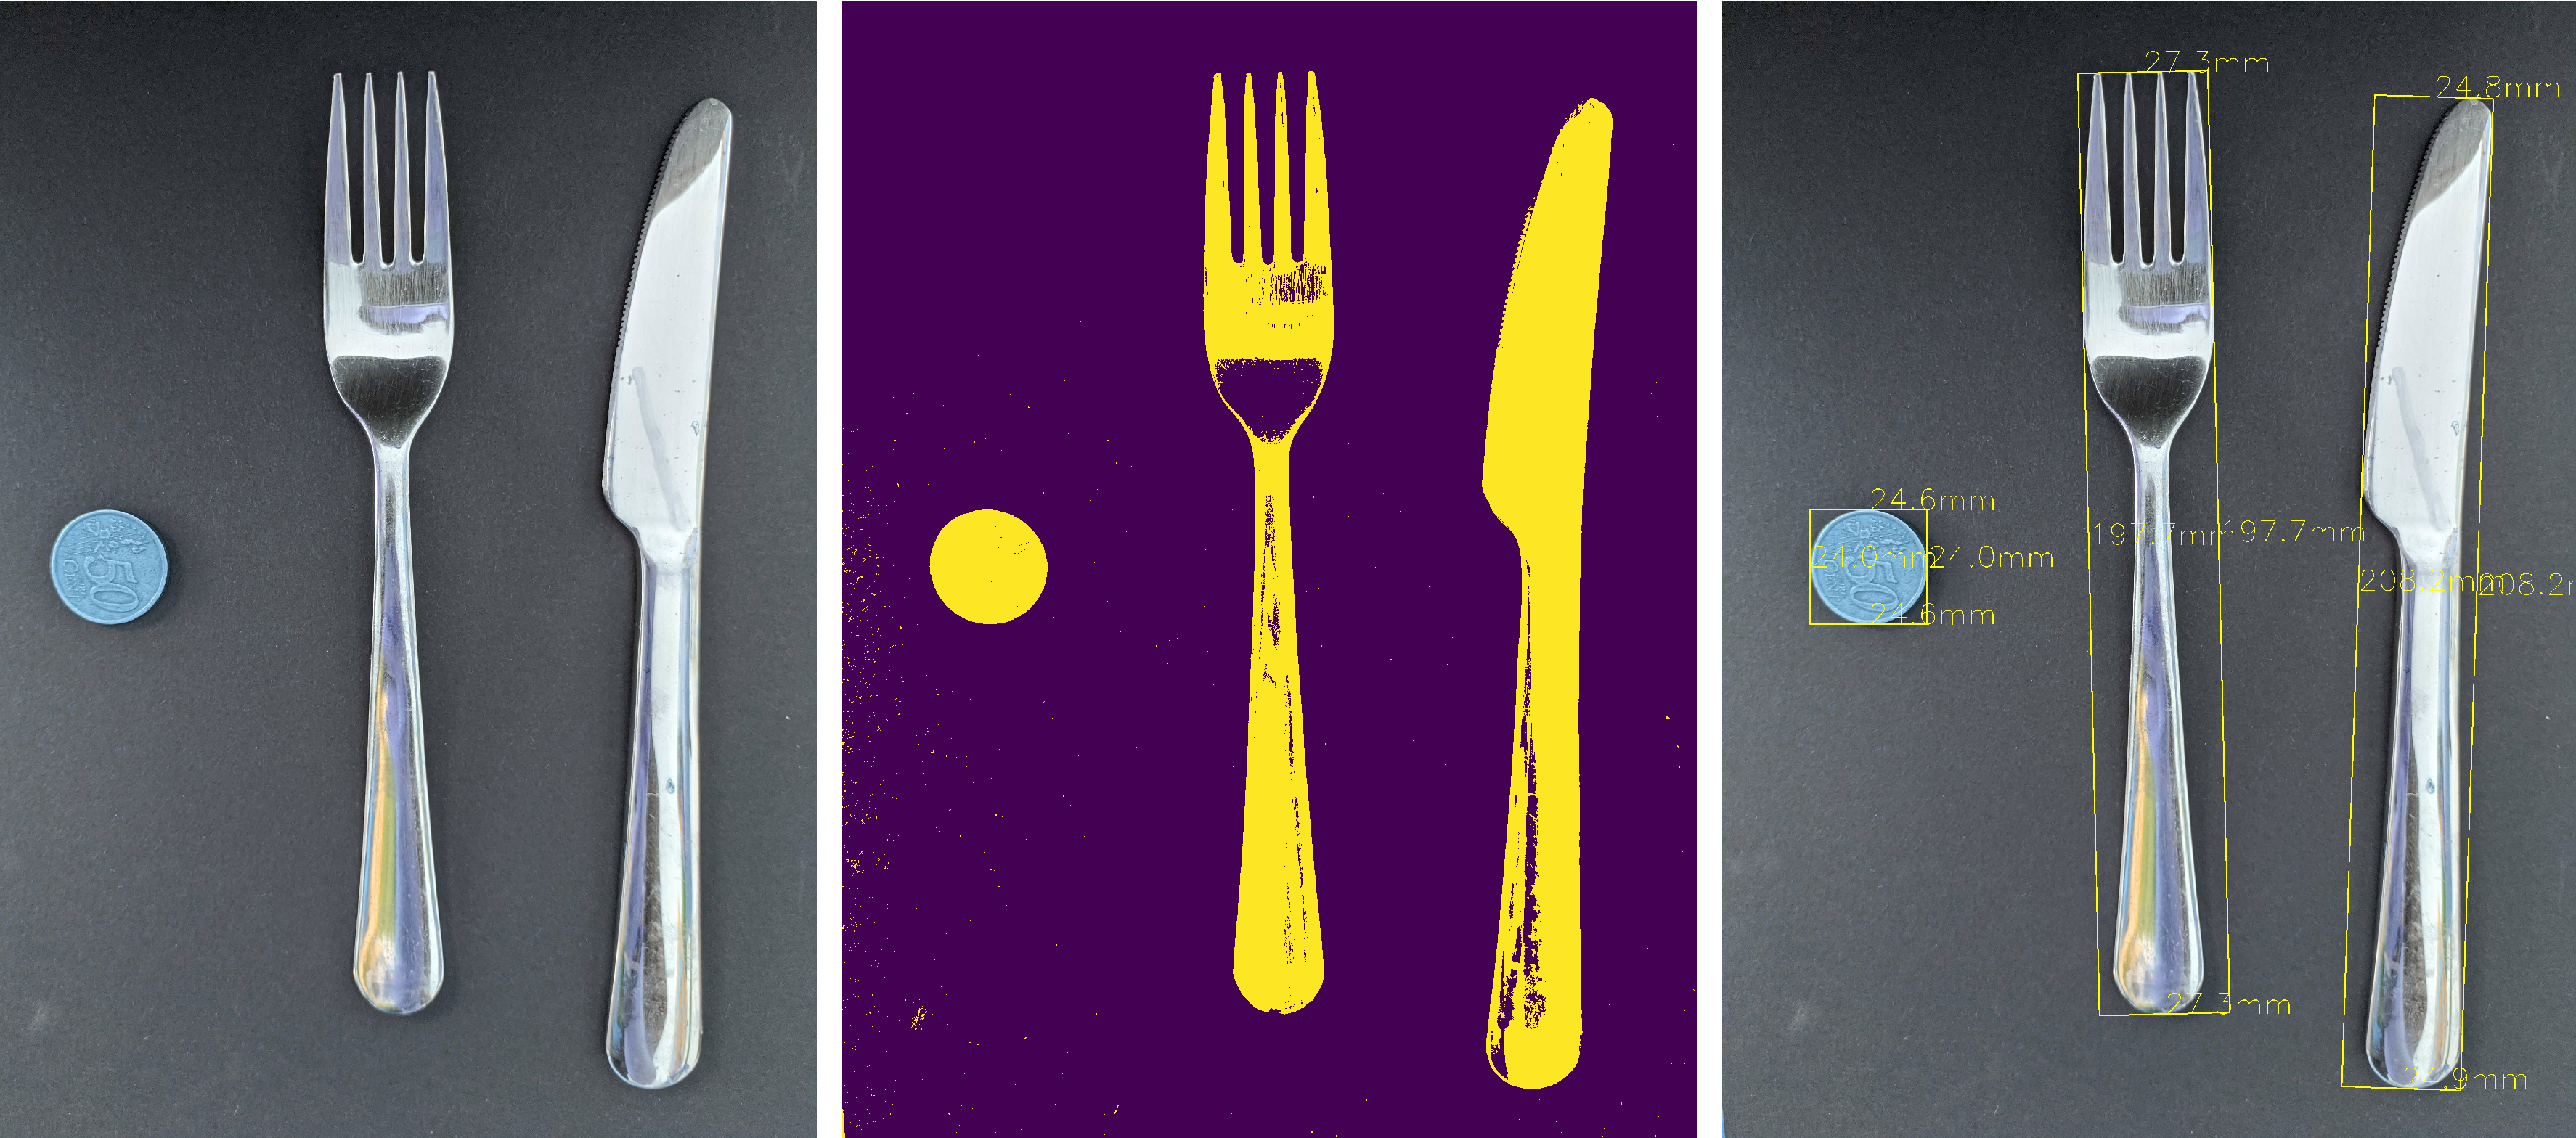
\includegraphics[scale=0.07	]{output.png}
	\caption[center]{Bild als Original (links), nach der Vorverarbeitung (Mitte), sowie nach der Vermessung (rechts). }
	\label{fig:intro}
\end{figure}


Das Bild soll im Anschluss an die Aufnahme mehrere Vorbereitungsschritte durchlaufen, bevor die eigentliche Objektvermessung stattfindet. Zunächst wird durch ein Schwellwertverfahren das Bild binarisiert. Dies ist notwendig, um in einem späteren Verarbeitungsschritt die Konturen der Objekte mit Hilfe des in \cite{Suzuki1985TopologicalSA} präsentierten Algorithmus finden zu können. Das binarisierte Bild wird im Anschluss durch einen Weichzeichner um grobe Körnungen und Unreinheiten bereinigt. 

Das vorverarbeitete Bild soll im Anschluss mit Hilfe von \cite{Suzuki1985TopologicalSA} nach Konturen durchsucht werden. Da uns nur die Gesamtlänge und Breite des Werkstücks interessiert, wird jeweils ein Rechteck mit der kleinst möglichen Fläche um die Konturen gespannt. Anhand der Entfernung benachbarter Eckpunkte der Rechtecke kann anschließend die Länge und Breite des Werkstücks in Pixel ausgerechnet werden. Um die gemessene Länge der Werkstücke von Pixel in Millimeter umwandeln zu können, wird ein Referenzobjekt im Bild platziert, dessen Maße bekannt sind. Hierbei soll ein Gegenstand mit gleichen Längen- und Breitenmaßen gewählt werden. Dadurch kann später geprüft werden, ob  alle Seiten des Referenzobjektes als gleich lang erkannt werden. Abweichungen von Länge und Breite des Referenzobjektes können somit als minimaler Messfehler angegeben werden. Wie in Abbildung \ref{fig:intro} zu sehen ist, wurde eine Münze als Referenzobjekt gewählt.

\section{Realisierung}

Alle Bilder wurden wie in Sektion \ref{sec:2} beschrieben mit Hilfe der Hauptkamera eines Google \emph{Pixel 2 XL Smartphones} \footnote{https://www.cnet.com/products/google-pixel-2-xl/specs/} mit einer Auflösung von 12.2 Megapixel aufgenommen. Als Bildhintergrund wurde ein mattschwarzer Karton, wie auf Abbildung \ref{fig:intro} (links) zu sehen ist, verwendet. Durch den dunklen Bildhintergrund sind die Schatten der Werkstücke weniger markant. Die Auswirkung des Schattenwurfs bei einem hellen Bildhintergrund ist exemplarisch auf Abbildung \ref{fig:shade} dargestellt. Insgesamt wurden 4 verschiedene Bilder mit 3 verschiedenen zu vermessenden Objekten fotografiert. Auf jedem Bild wurde ein Referenzobjekt mit bekannter Größe platziert. Es wurde bewusst darauf geachtet, dass sich die Ausrichtung der Objekte in den Bildern unterscheidet, um einer Überanpassung des Messalgorithmus entgegenzuwirken.

\begin{figure}
	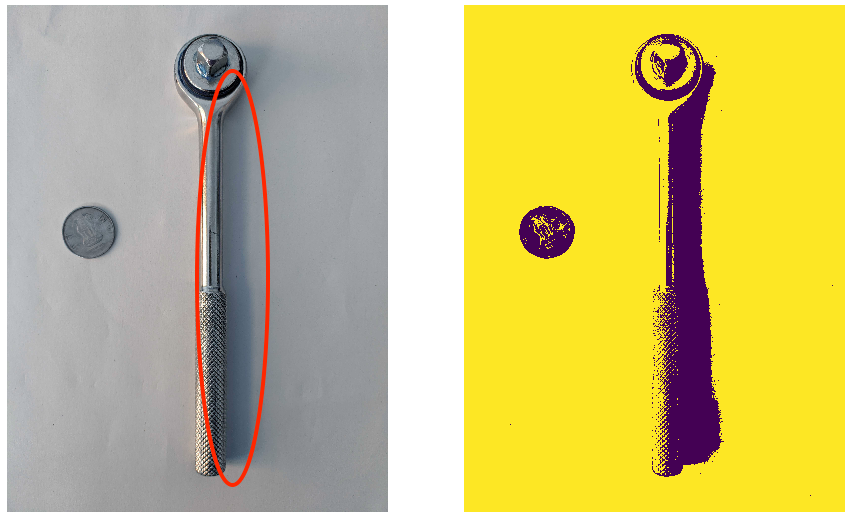
\includegraphics[scale=0.25]{bad_shade_white_background.png}
	\caption[center]{Die Auswirkungen des Schattens bei hellem Bildhintergrund}
	\label{fig:shade}
\end{figure}

\begin{figure}
	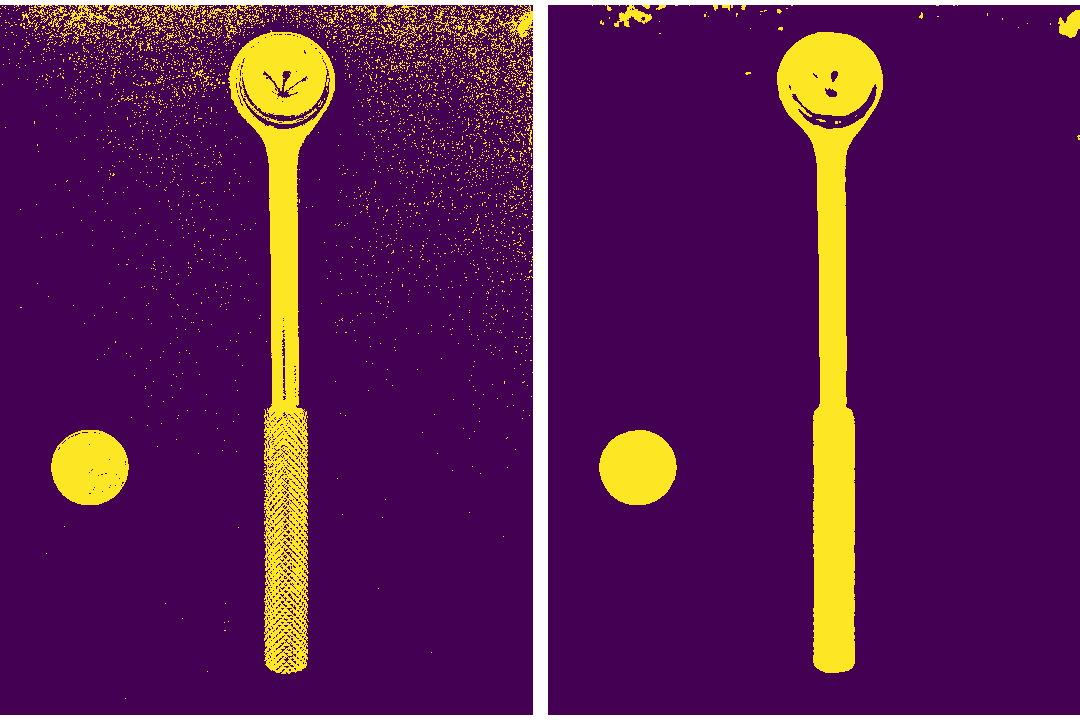
\includegraphics[scale=0.2]{blurr}
	\caption[center]{Das Binärbild vor (links) und nach (rechts) der Anwendung des Medianfilters}
	\label{fig:blurr}
\end{figure}

Das entworfene Konzept zur Vorverarbeitung und Vermessung des Eingabebildes wurde mit der \emph{OpenCV}-Bibliothek in Python umgesetzt. Im folgenden Codeausschnitt sind die implementierten Vorverarbeitungsschritte aufgeführt.

\begin{lstlisting}[language=Python, caption=Vorverarbeitung]
import cv2

raw_img = cv2.imread("image.jpg")
grey = cv2.cvtColor(raw_img, cv2.COLOR_BGR2GRAY)
_ , thresh = cv2.threshold(grey, 127, 255, 0)
median_blurred = cv2.medianBlur(thresh, 11)

\end{lstlisting}
In Zeile 4 wird das Bild zunächst vom RGB-Format in ein Graustufenbild umgewandelt. Dieser Schritt wird von  \emph{OpenCV} empfohlen, um das Bild anschließend in ein Binärbild umzuwandeln. Die Überführung in das Binärformat passiert mit dem Aufruf aus Zeile 5. Der Schwellwert-Parameter für das Verfahren wurde empirisch auf 127 festgelegt. Als finaler Vorbereitungsschritt wird in Zeile 6 noch mit Hilfe des Medianfilters das Bild von Ausreißerpixel befreit (siehe Abbildung \ref{fig:blurr}). Auch die Filtergröße des Medianfilters wurde empirisch auf 11 festgelegt.

Das Bild wird im Anschluss der Vorverarbeitung mit der \emph{OpenCV}-Funktion \emph{findContours()} nach Konturen abgesucht. Wie bereits oben angedeutet, implementiert die Funktion den Algorithmus aus \cite{Suzuki1985TopologicalSA}. Es werden nur die Flächenmäßig größten \(n\) gefunden Konturen weiter verarbeitet. \(n\) entspricht hierbei der Anzahl im  Bild enthaltener Werkstücke und muss vor der Skriptausführung als Parameter festgelegt werden. Im nächsten Schritt werden mit Hilfe der \emph{minAreaRect()}-Funktion \(n\) Rechtecke mit minimaler Fläche kalkuliert, die die größten \(n\) Konturen umfassen. Dadurch kann im nachfolgenden Schritt die euklidische Distanz zwischen den Eckpunkten der minimalen Rechtecke kalkuliert werden. Zwei benachbarte gefundene Kanten entsprechen jeweils der Länge und Breite eines Werkstücks in Pixeln. Die Umrechnung der Kantenlängen von Pixel in Millimeter erfolgt wie oben beschrieben durch das Referenzobjekt.

Die Ausgabe der Messergebnisse erfolgt durch die Einblendung von \emph{Boundingboxen} inklusive der Kantenlängen in Millimeter in das Originalbild (siehe Abbildung \ref{fig:intro} rechts).

\section{Ergebnisse}
Um die Genauigkeit der Vermessung beurteilen zu können wurden die Messergebnisse des Messers (Abbildung \ref{fig:intro}) auf verschiedenen Bildern verglichen. Die Länge des Messers wurde auf drei verschiedenen Bildern im Mittel mit 20,45 cm und einer Standardabweichung von 0,44 cm vermessen. Die tatsächliche Länge des Messers beträgt 20,6 cm. Der durchschnittliche Messfehler für die Länge des Messers beträgt damit 0.7\%. Der durchschnittliche Gesamtmessfehler aller Objekte auf den 3 Bildern beträgt 1.1\%.
Außerdem wurde das Verfahren auf eine Überanpassung auf die anfangs aufgenommenen drei Bilder und der darauf befindlichen Objekte untersucht. Hierzu wurde nach Abschluss der Implementierung ein weiteres Bild mit einem neuen Objekt (Löffel) aufgenommen und vermessen. Auch auf diesem Bild konnte der Gegenstand erfolgreich mit einem vergleichbaren Fehler vermessen werden.

\section{Fazit}
Mit dem vorgestellten Verfahren konnte eine Vermessung von Objekten mit spiegelnden Eigenschaften implementiert werden. Optimierungsbedarf besteht bei der Ausrichtung der minimalen Rechtecke, die um gefundene Konturen gespannt werden. Die Rechtecke verlaufen nicht immer parallel zu den längsten Kanten des Messstücks und verursachen dadurch einen Messfehler. Um die Generalisierbarkeit des Verfahrens zu verbessern, könnte noch ein Schritt implementiert werden, der die empirisch festgelegten Schwellwerte für die Binarisierung automatisch wählt und anpasst.

\bibliographystyle{asmems4}

% Here's where you specify the bibliography database file.
% The full file name of the bibliography database for this
% article is asme2e.bib. The name for your database is up
% to you.
\bibliography{asme2e}

\end{document}
